\subsection{Strategy}
\label{strategy}

\textbf{Scopo}: Comportamentale \\
\textbf{Raggio d'azione}: Oggetti

\paragraph{Definizione} Il pattern permette di definire una famiglia di algoritmi, incapsularli singolarmente e renderli interscambiabili. Strategy consente all'algoritmo di variare indipendentemente dai Client che lo utilizzano.

A differenza di Template Method (\ref{template-method}), in cui si congela l'algoritmo per risolvere il problema a seconda del tipo di specifica, Strategy cambia l'algoritmo a seconda del tipo concreto.

\paragraph{Motivazione} Esistono molti algoritmi per spezzare un flusso di testo in righe, ma cablare tutti questi algoritmi nelle classi che li richiedono non è desiderabile per diverse ragioni: i client che necessitano di interruzioni di riga diventano più complessi se includono il codice di interruzione di riga, rendendoli più grandi e difficili da mantenere, specialmente se supportano algoritmi multipli di interruzione di riga; algoritmi diversi saranno appropriati in momenti diversi e non vogliamo supportare algoritmi multipli di interruzione di riga se non li usiamo tutti; è difficile aggiungere nuovi algoritmi e variare quelli esistenti quando l'interruzione di riga è una parte integrale di un client. 

\begin{figure}[H]
    \centering
    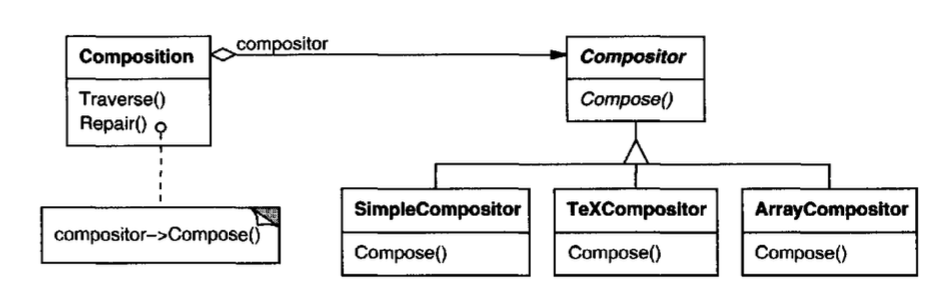
\includegraphics[width=0.75\linewidth]{assets/pattern/strategy/strategy-esempio.png}
\end{figure}

Possiamo evitare questi problemi definendo classi che incapsulano diversi algoritmi di interruzione di riga, dove un algoritmo incapsulato in questo modo è chiamato strategia. Supponiamo che una classe Composition sia responsabile di mantenere e aggiornare le interruzioni di riga del testo visualizzato in un visualizzatore di testo: le strategie di interruzione di riga non sono implementate dalla classe Composition, invece sono implementate separatamente da sottoclassi della classe astratta Compositor, dove le sottoclassi Compositor implementano strategie diverse come SimpleCompositor che implementa una strategia semplice che determina le interruzioni di riga una alla volta, TeXCompositor che implementa l'algoritmo TeX per trovare interruzioni di riga cercando di ottimizzare le interruzioni globalmente un paragrafo alla volta, e ArrayCompositor che implementa una strategia che seleziona interruzioni così che ogni riga abbia un numero fisso di elementi. Una Composition mantiene un riferimento a un oggetto Compositor e ogni volta che una Composition riformatta il suo testo, inoltra questa responsabilità al suo oggetto Compositor, dove il client di Composition specifica quale Compositor dovrebbe essere usato installando il Compositor desiderato nella Composition. 

\newpage

\paragraph{Applicabilità} Il pattern Strategy è utile quando:

\begin{itemize}
    \item Si desidera utilizzare diverse varianti di un algoritmo all'interno di un oggetto ed essere in grado di passare da un algoritmo all'altro a runtime.
    \item Si hanno molte classi simili che differiscono solo nel modo in cui eseguono alcuni comportamenti (queste classi spesso contengono istruzioni condizionali massicce per passare da un'algoritmo all'altro).
\end{itemize}

In più permette di isolare la logica di business di una classe dai dettagli di implementazione degli algoritmi che potrebbero non essere così importanti nel contesto di tale logica.

\begin{figure}[H]
    \centering
    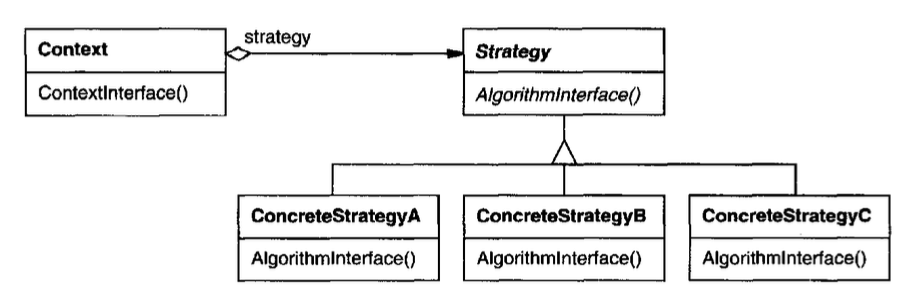
\includegraphics[width=0.75\linewidth]{assets/pattern/strategy/strategy-struttura.png}
    \caption{Class Diagram del pattern Strategy}
\end{figure}

\paragraph{Struttura} Il pattern è composto da:
\begin{itemize}
    \item \textbf{Context}: mantiene un riferimento a una delle ConcreteStrategy e comunica con questo oggetto solo tramite l’interfaccia Strategy.
    \item \textbf{Strategy}: interfaccia comune a tutte le ConcreteStrategy. Dichiara un metodo che il contesto utilizza per eseguire una strategia.
    \item \textbf{ConcreteStrategy}: implementano diverse varianti di un algoritmo utilizzato dal Context.
    \item \textbf{Client}: crea un oggetto ConcreteStrategy e lo passa al Context, il quale espone un setter che consente ai Client di sostituire la Strategy associata al Context a runtime.
\end{itemize}

\begin{figure}[H]
    \centering
    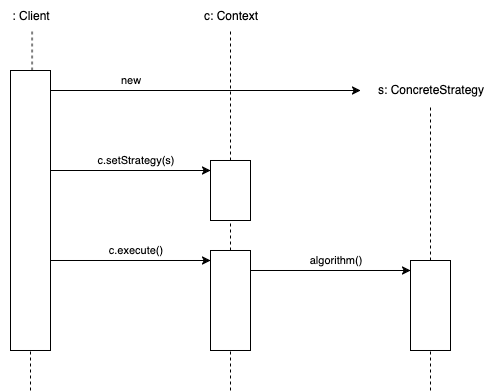
\includegraphics[width=0.5\linewidth]{assets/pattern/strategy/strategy-sequence.drawio.png}
    \caption{Sequence Diagram del pattern Strategy}
\end{figure}

\paragraph{Conseguenze} Il pattern Strategy consente quindi di:
\begin{itemize}
    \item Definire famiglie di algoritmi correlati;
    \item Avere un'alternativa al subclassing;
    \item Eliminare istruzioni condizionali;
    \item Scegliere tra varie implementazioni;
\end{itemize}

I Client devono essere consapevoli delle diverse strategie implementate. Esiste un overhead di comunicazione tra Strategy e Context. In più aumenta il numero di oggetti istanziati.

\paragraph{Pattern correlati} Può essere considerato come un'estensione del pattern State (\ref{state}), entrambi sono basati sulla \textbf{composizione}: modificano il comportamento del contesto delegando parte del lavoro agli oggetti helper. Sebbene, il pattern State non limiti le dipendenze tra stati concreti, consentendo loro di alterare a piacimento lo stato del contesto.


\newpage